\documentclass[10pt]{standalone}
\usepackage[utf8]{inputenc}
\usepackage{pgf,tikz,pgfplots}
\pgfplotsset{compat=1.15}
\usepackage{mathrsfs}
\usetikzlibrary{arrows}
\pagestyle{empty}
\begin{document}
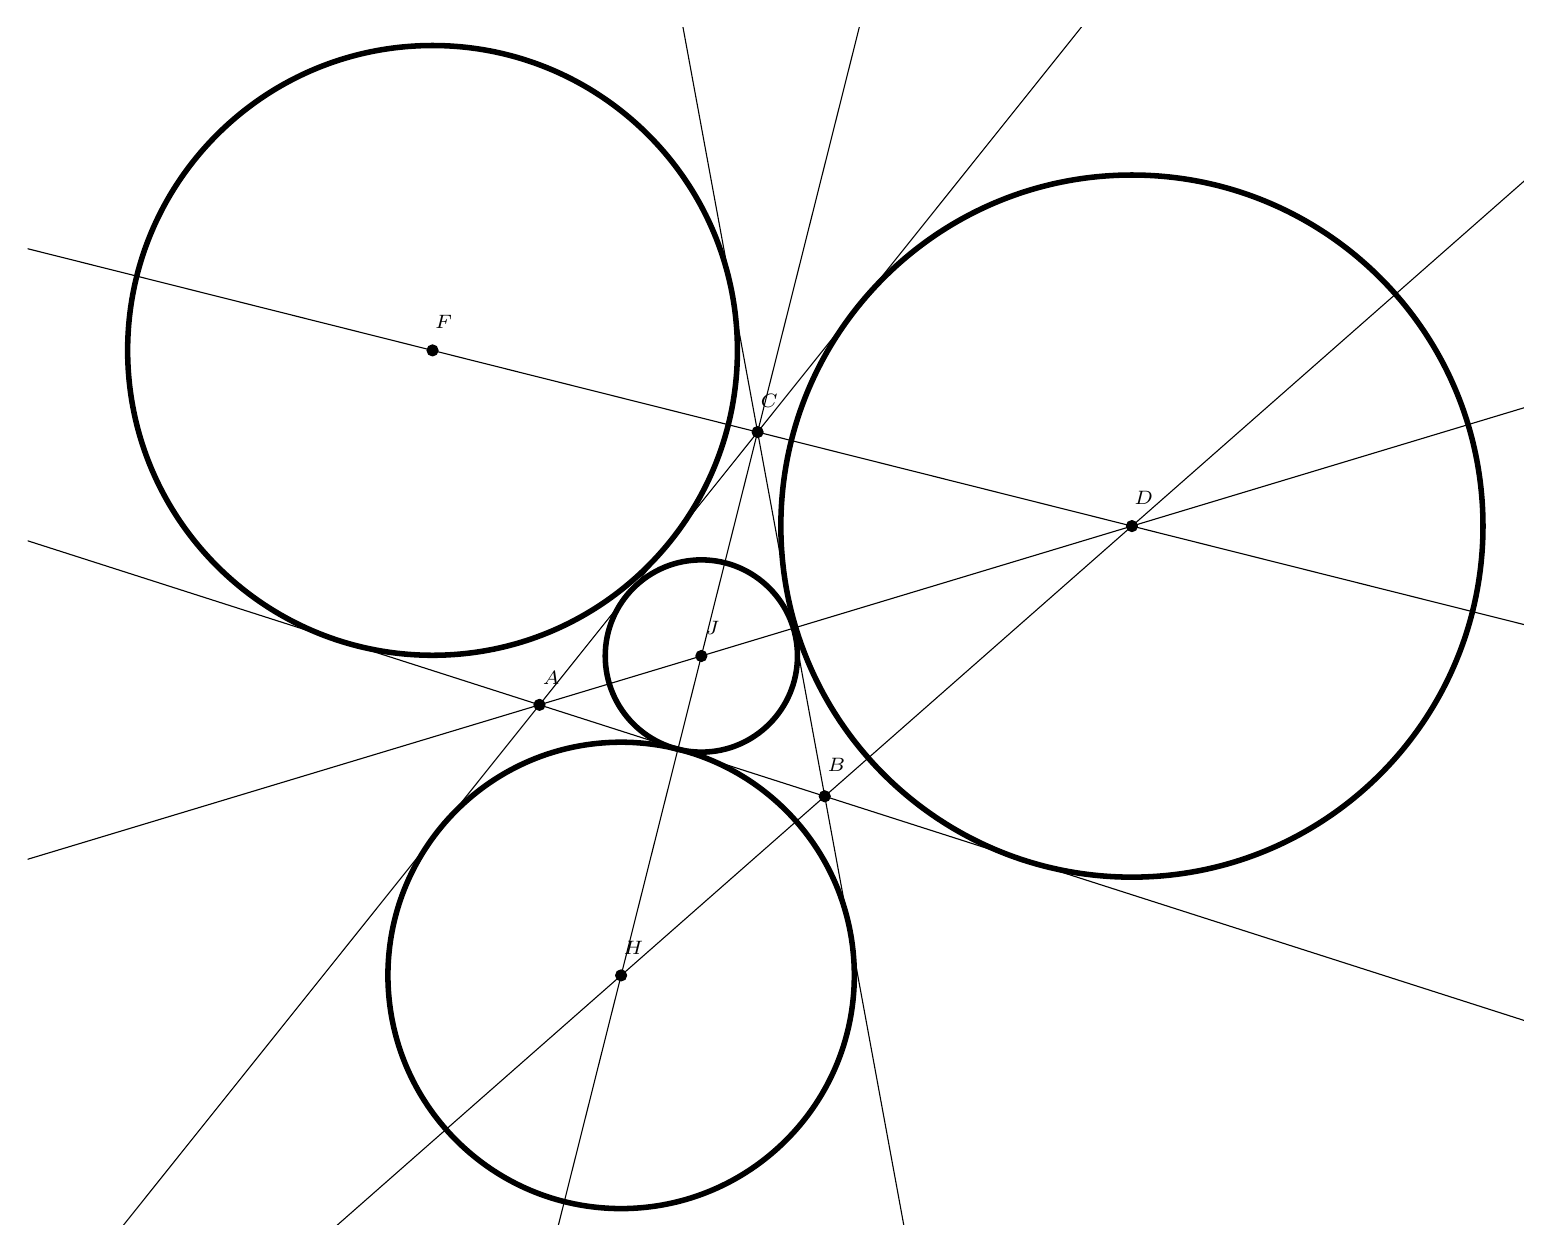
\begin{tikzpicture}[line cap=round,line join=round,>=triangle 45,x=1.0cm,y=1.0cm]
%\begin{axis}[
%x=1.0cm,y=1.0cm,
%axis lines=middle,
%%ymajorgrids=true,
%%xmajorgrids=true,
%xmin=-6.0,
%xmax=12.5,
%ymin=-6.6,
%ymax=8.6,
%ticks=none,
%]
\clip(-6.5,-6.6) rectangle (12.5,8.6);
\draw [domain=-6.5:13.5] plot(\x,{(-0.--3.464396052718255*\x)/2.770130751191044});
\draw [domain=-6.5:13.5] plot(\x,{(--15.767610844916462-4.625656769270266*\x)/0.8526556256719391});
\draw [domain=-6.5:13.5] plot(\x,{(-0.--1.1612607165520117*\x)/-3.622786376862983});
\draw [domain=-6.5:13.5] plot(\x,{(-0.-0.28887520413651546*\x)/-0.9573667617141753});
\draw [domain=-6.5:13.5] plot(\x,{(--3.2646741596274698-0.6604688485205706*\x)/-0.7508534478404635});
\draw [domain=-6.5:13.5] plot(\x,{(--4.034892461887093-0.24362882555343285*\x)/0.9698685454016205});
\draw [domain=-6.5:13.5] plot(\x,{(-1.842635940654259--0.9698685454016205*\x)/0.24362882555343285});
\draw [line width=2.pt] (7.523905849169923,2.270258301208685) circle (4.45854360090309cm);
\draw [line width=2.pt] (-1.3582611636615378,4.501438936940597) circle (3.8719996160129293cm);
\draw [line width=2.pt] (1.036771011839885,-3.435982362041759) circle (2.96160697641247cm);
\draw [line width=2.pt] (2.0556962169911097,0.6202843968206011) circle (1.2206781158240956cm);
\begin{scriptsize}
\draw [fill=black] (0.,0.) circle (2.0pt);
\draw[color=black] (0.1482147022498305,0.34154482369477995) node {$A$};
\draw [fill=black] (3.622786376862983,-1.1612607165520117) circle (2.0pt);
\draw[color=black] (3.7720011113555727,-0.7669074896787401) node {$B$};
\draw [fill=black] (2.770130751191044,3.464396052718255) circle (2.0pt);
\draw[color=black] (2.919345485683633,3.8587492795915264) node {$C$};
\draw [fill=black] (7.523905849169923,2.270258301208685) circle (2.0pt);
\draw[color=black] (7.672900598804695,2.6223986223672155) node {$D$};

\draw [fill=black] (-1.3582611636615378,4.501438936940597) circle (2.0pt);
\draw[color=black] (-1.2160342988252724,4.860619639756054) node {$F$};
;
\draw [fill=black] (1.036771011839885,-3.435982362041759) circle (2.0pt);
\draw[color=black] (1.1927178436979562,-3.0903940696347725) node {$H$};
%\draw [fill=black] (1.7583038412541079,-0.5636129117773052) circle (2.0pt);
%\draw[color=black] (1.9174751255191047,-0.21268133299198008) node {$I$};

\draw [fill=black] (2.0556962169911097,0.6202843968206011) circle (2.0pt);
\draw[color=black] (2.1945882038624847,0.9810365429487338) node {$J$};

\end{scriptsize}
%\end{axis}
\end{tikzpicture}
\end{document}